\documentclass[../main.tex]{subfiles}

\begin{document}

Most \gls{cryoem} image processing suites such as Relion\cite{scheres2021}, Cryosparc\cite{cryosparc}, Cistem\cite{grigorieff2018} and Xmipp\cite{sorzano2021} implement a refinement step in which a 3D model is iteratively improved. This process should converge to a high resolution solution which is compatible with the provided images. 

The input for this step is a large set of noisy images presumably containing the projection of a particle. A low-resolution estimation of the volume is also provided (initial volume).

Input images are not clean, in fact they have many artefacts. Firstly, they have been ``coloured'' in frequency space by a transfer function known as \gls{ctf}. This transfer function has been estimated in previous steps, so it does not need to be deduced (although it can be fine-tuned). Moreover, the particle is not perfectly centered in the image box. Last but not least, the images contain a vast amount of noise. In fact, the \gls{snr} is in the order of $xx \si{\decibel}$. The \gls{psd} of the noise roughly resembles to pink noise. However, the exact \gls{psd} of the noise is unknown and should also be estimated from data.

Before attempting to reconstruct the 3D structure of the specimen, the projection directions of each of the images need to be deduced in a process known as particle alignment. This is a computationally expensive task and much effort has been put into it to reduce the amount of time expended on this process. 

The alignment process relies on projecting the current volume from multiple perspectives, somewhat mimicking the microscope's behaviour. Then, each of the particle images is searched across all simulated projections, considering in-plane transformations (rotations and translations). The actual similarity metric used for matching varies across the existing solutions. 

Once a best match has been found, the projection parameters of the selected reference image and its best transform can be assigned to the experimental one. This enables using the experimental images to reconstruct a new volume, potentially with a higher resolution. This last volume can be used as the initial volume for the next iteration. This cycle is illustrated in the figure \ref{fig:3:refinement}. 

\begin{figure}[h]
    \centering
    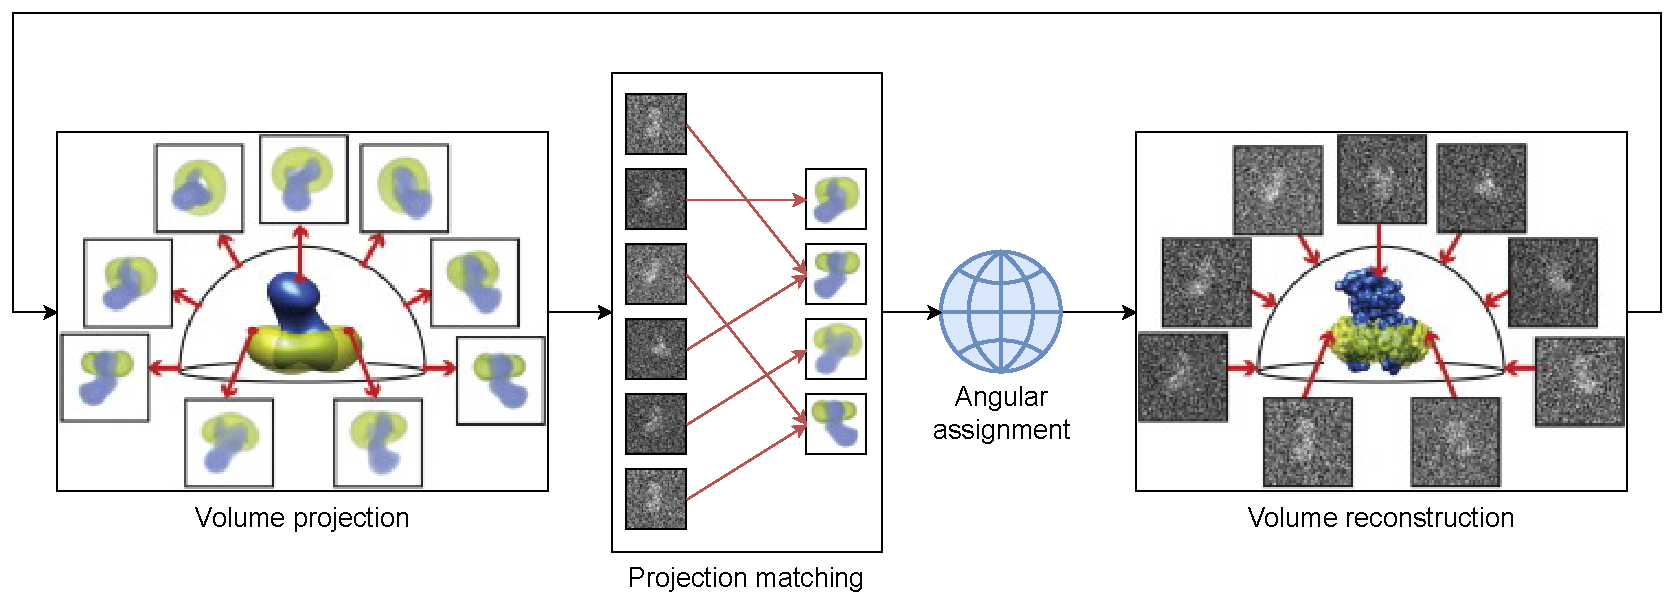
\includegraphics[width=\textwidth]{SPA/refinement}\\
    Images obtained from: \cite{nogales2015}
    \caption{Typical refinement cycle}
    \label{fig:3:refinement}
\end{figure}

\subsection{Projection gallery generation}
The projection gallery represents a set of ``views'' of the input volume from relevant directions. This collection of images is generated by projecting the initial volume in the same way that a \gls{tem} microscope would do. This enables performing comparisons between experimental and generated images. 

\subsubsection{Projection procedure}
In rough terms, \glspl{tem} fire a electron beam through the sample and capture the ``shadow'' of its electron density. In other words, areas where the beam encounters electrons will appear dim. This process is illustrated in the figure \ref{fig:3:projection}. Nevertheless images are usually complemented so that bright areas relate to the presence of matter.

\begin{figure}[h]
    \centering
    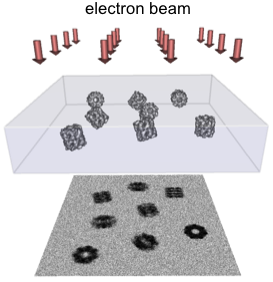
\includegraphics[width=.5\textwidth]{SPA/projection_reconstruction/acquisition}\\
    Images obtained from: \cite{greg}
    \caption{TEM image acquisition}
    \label{fig:3:projection}
\end{figure}

This behaviour is mathematically known as the X-Ray transform, which is a particularisation to 3 dimensions of the Radon's transform. As described in the equation \eqref{eq:3:xray}, this transform consists in computing the integral across a set of parallel lines normal to the projection plane.

\begin{equation}\label{eq:3:xray}
    Xf(L) = \int_L f
\end{equation}

This computation can be significantly accelerated using the Fourier Central Slice Theorem. This theorem states that projecting a $N$-dimensional function to $N-1$ dimensions and then taking its \gls{ft} is equivalent to computing the $N$-dimensional \gls{ft} and then extracting the central hyperplane normal to the projection direction. This equivalence is shown in the figure \ref{fig:3:3dfourier}. Therefore, a set of projections can be generated by extracting 2D planes from the 3D \gls{ft} of the input volume and then computing their \gls{ift}.

\begin{figure}[h]
    \centering
    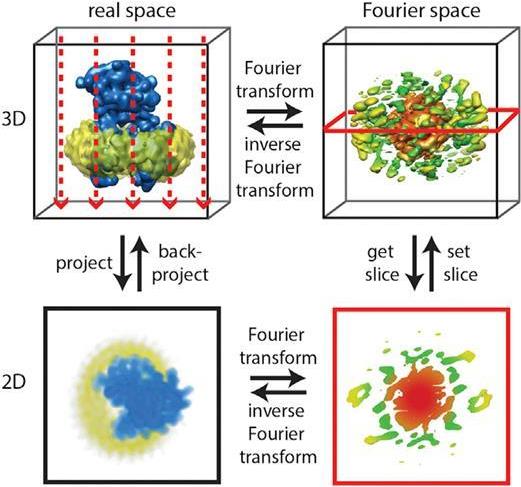
\includegraphics[width=.5\textwidth]{SPA/3d_fourier_reconstruction}\\
    Images obtained from: \cite{nogales2015}
    \caption{Fourier Slice Theorem illustration for 3D}
    \label{fig:3:3dfourier}
\end{figure}

Note that when using this approach, only one 3D \gls{fft} is computed, and then for each projection direction, a 2D central slice is extracted from it, which contains the 2D \gls{ft} of the projected image. More often than not, the following steps are performed in Fourier space, so computing the \gls{ift} of the slices is not needed.

\subsection{Projection matching and angular assignment}
Each of the input particles needs to be searched across the projections generated in the prior section, also considering all possible in plane transformations (rotations and shifts). 

This search can be either local or global. For global searches, the projection gallery is generated with a uniform spacing between projection angles and all their in-plane transforms are also generated with a regular interval. Then, for each experimental image all combinations are tested to find a best match. However, as the target resolution increases, the sampling rate of the parameters also needs to be increased. This makes global searches unfeasible beyond low-resolution targets. Therefore, for high resolution, local searches are used. This means that images are only sampled around a narrow range centred in their previous assignment, significantly increasing thoughput. However, local searches need to be applied with precaution, as they involve the risk of falling in local minimas.

When comparing reference images and experimental images, the \gls{ctf} needs to be considered. Experimental images have been ``coloured´´ with a characteristic transfer function induced by the microscope. As opposed to this, the reference gallery was generated artificially without considering any frequency response. Therefore, this transfer function needs to be addressed before attempting to compare images to one another. Most of the current implementations choose to filter the reference images with the experimental's estimated \gls{ctf}. Note that the \gls{ctf} may vary from particle to particle. Therefore, for each particle, the \gls{ctf} needs to be re-applied to the reference gallery.

In essence, this step can be seen as a \gls{knn} problem with $k=1$. This means that we have a large set of images composed of all the projections of the current volume and its in plane transformations. For each experimental image we want to find the most similar one, this is, the image which minimises some distance metric.

The problem can be mathematically expressed with the expression \eqref{eq:3:minimization} where $C$ is the estimated \gls{ctf} of the experimental image $I_{exp}$. $\Phi$ is a projection $\mathbb{R}^3 \mapsto \mathbb{R}^2$. Finally, $V$ is the reference volume. The actual distance function used depends on the implementation. All of $C$, $V$ and $I_{exp}$ remain constant for a given search. Therefore, only the projection parameters regarding $\Phi$ need to be optimised.

\begin{equation}\label{eq:3:minimization}
    \min_\Phi \text{dist}(C\Phi V, I_{exp})
\end{equation}

The distance function is used to evaluate similarity between pairs of reference and experimental images. As mentioned earlier, the election of this function may vary across different implementations. More often than not, this distances are calculated in Fourier space, as high frequencies contain little information due to low levels of \gls{snr}. This allows to compute distances in a reduced set of coefficients corresponding to low frequencies, allowing more efficient computations.

\begin{itemize}
    \item \textbf{Euclidean}: The euclidean distance is defined as the square root of the sum of squared coefficients. The square root part can be ignored, as it is not necessary for comparisons. In the equation \eqref{eq:3:euclidean2} it is defined for complex numbers, necessary for comparing in Fourier space.

    \begin{equation}\label{eq:3:euclidean2}
        dist_{\text{L2}}(x, y)^2 = (x-y)^H \cdot (x-y)
    \end{equation}
    
    \item \textbf{Weighted euclidean}: The weighted euclidean distance features a weight matrix to give more importance to some coefficients. In the case of Relion\cite{scheres2021} and Cryosparc\cite{cryosparc} this weights are derived from the Maximum Likelihoods Estimation. In essence, the weights correspond to the inverse of the noise variance, this is, the inverse of the noise power. Therefore, \gls{psd} of the noise needs to be estimated.
    
    \begin{equation}\label{eq:3:euclidean2_weighted}
        dist_{\text{L2,W}}(x, y)^2 = (x-y)^H \cdot W \cdot (x-y)
    \end{equation}
    
    \item \textbf{Pearson correlation}: Perarson correlation is not a distance metric but a similarity metric. Nevertheless it can be easily converted to a distance function applying a monotonically decaying function ($1-x$, $1/x$, $e^{-x}$, \dots). It is defined in the equation \eqref{eq:3:pearson}
    
    \begin{equation}\label{eq:3:pearson}
        \rho_{x,y} =    \frac{
                        (x-\bar{x})^T(y-\bar{y})
                        }{
                        \sqrt{(x-\bar{x})^T(x-\bar{x}) \cdot (y-\bar{y})^T(y-\bar{y})}
                        }
    \end{equation}
\end{itemize}

Finally, once a best reference match is found, the projection parameters and in-plane transform of the reference is assigned to the experimental image, as presumably it has been captured in such orientation.

\subsection{3D reconstruction}
The 3D reconstruction step consists in building a 3D electron density map using the angular-assigned experimental particles. Originally, this was performed using back-projection algorithms. Later this was replaced by the \gls{art} method, which approaches the reconstruction problem as a Least Squares problem. Current solutions rely on the Fourier Central Slice theorem, which was previously.

\subsubsection{ART reconstruction}
\Gls{art} is a iterative reconstruction method. It formulates the reconstruction problem as a linear equation $Ax = b$ where $x$ is the vector encoding the reconstructed volume, $b$ is the set of experimental images and $A$ is derived from the projection directions. Then, the problem can be seen as a \gls{ls} problem trying to solve for $x$. In practice, $A$ is too large to be solved the conventional \gls{ls} equation. Therefore, a iterative gradient descent is used. As \gls{ls} is a convex problem the iterative method is guaranteed to find the global minima.

\subsubsection{Fourier Reconstruction}
Earlier, it has been stated that the Fourier transform of a 2D projection is equivalent to taking a 2D central slice from the 3D \gls{ft} of the volume. Fourier reconstruction leverages this fact by filling the 3D Fourier space with the appropriately oriented 2D Fourier transforms of the experimental images. Assuming that projections from all possible directions have been provided, the whole 3D Fourier space is defined, which means that the volume can be determined by computing the \gls{ift}. This principle is illustrated in the figure \ref{fig:3:3dfourier}.

\subsection{Multi-reference refinement}
The refinement algorithms rely on the assumption that all input particles belong to the same structure. However, this is not always true, as the dataset might be heterogeneous. This heterogeneity can be either discrete or continuous. 

The continuous heterogeneity relates to flexible macromolecules. These macromolecules have a certain amount of freedom to deform. Therefore, when projecting them, no single conformation can be attributed to the dataset. The study of these kind of proteins though \gls{cryoem} is a novel field which is currently under study.

Contrary to this, discrete heterogeneity involves a discrete amount of conformations in the dataset. For instance, a biologist may want to test how a particular ligand binds to the protein. In that case, it is reasonable to consider that some of the input particles may come from a structure with the ligand attached, whilst some others won't have it.

The most common way to solve discrete heterogeneity is to generalise the refinement algorithm to $N$ volumes. This is done by enabling multiple projection gallery inputs to the projection matching stage. Here, not only the projection parameters need to be considered, but also the reference volume. Then, each of the volumes can be reconstructed with the particles that were classified as such.

Although the working principle of multi-reference refinement is simple, there are many problems associated to it. Firstly, several input volumes need to be provided. These volumes have to be somewhat different so that the algorithm is able to converge to distinct volumes. Additionally, a problem known as attraction may appear. This problem is related to a class being able to gather increasingly more particles in each iteration, so that the other volumes are degraded and diverge. This last problem is usually solved by penalising the cost function for very populated classes.

\end{document}
